\begin{figure*}[t]
  \centering
   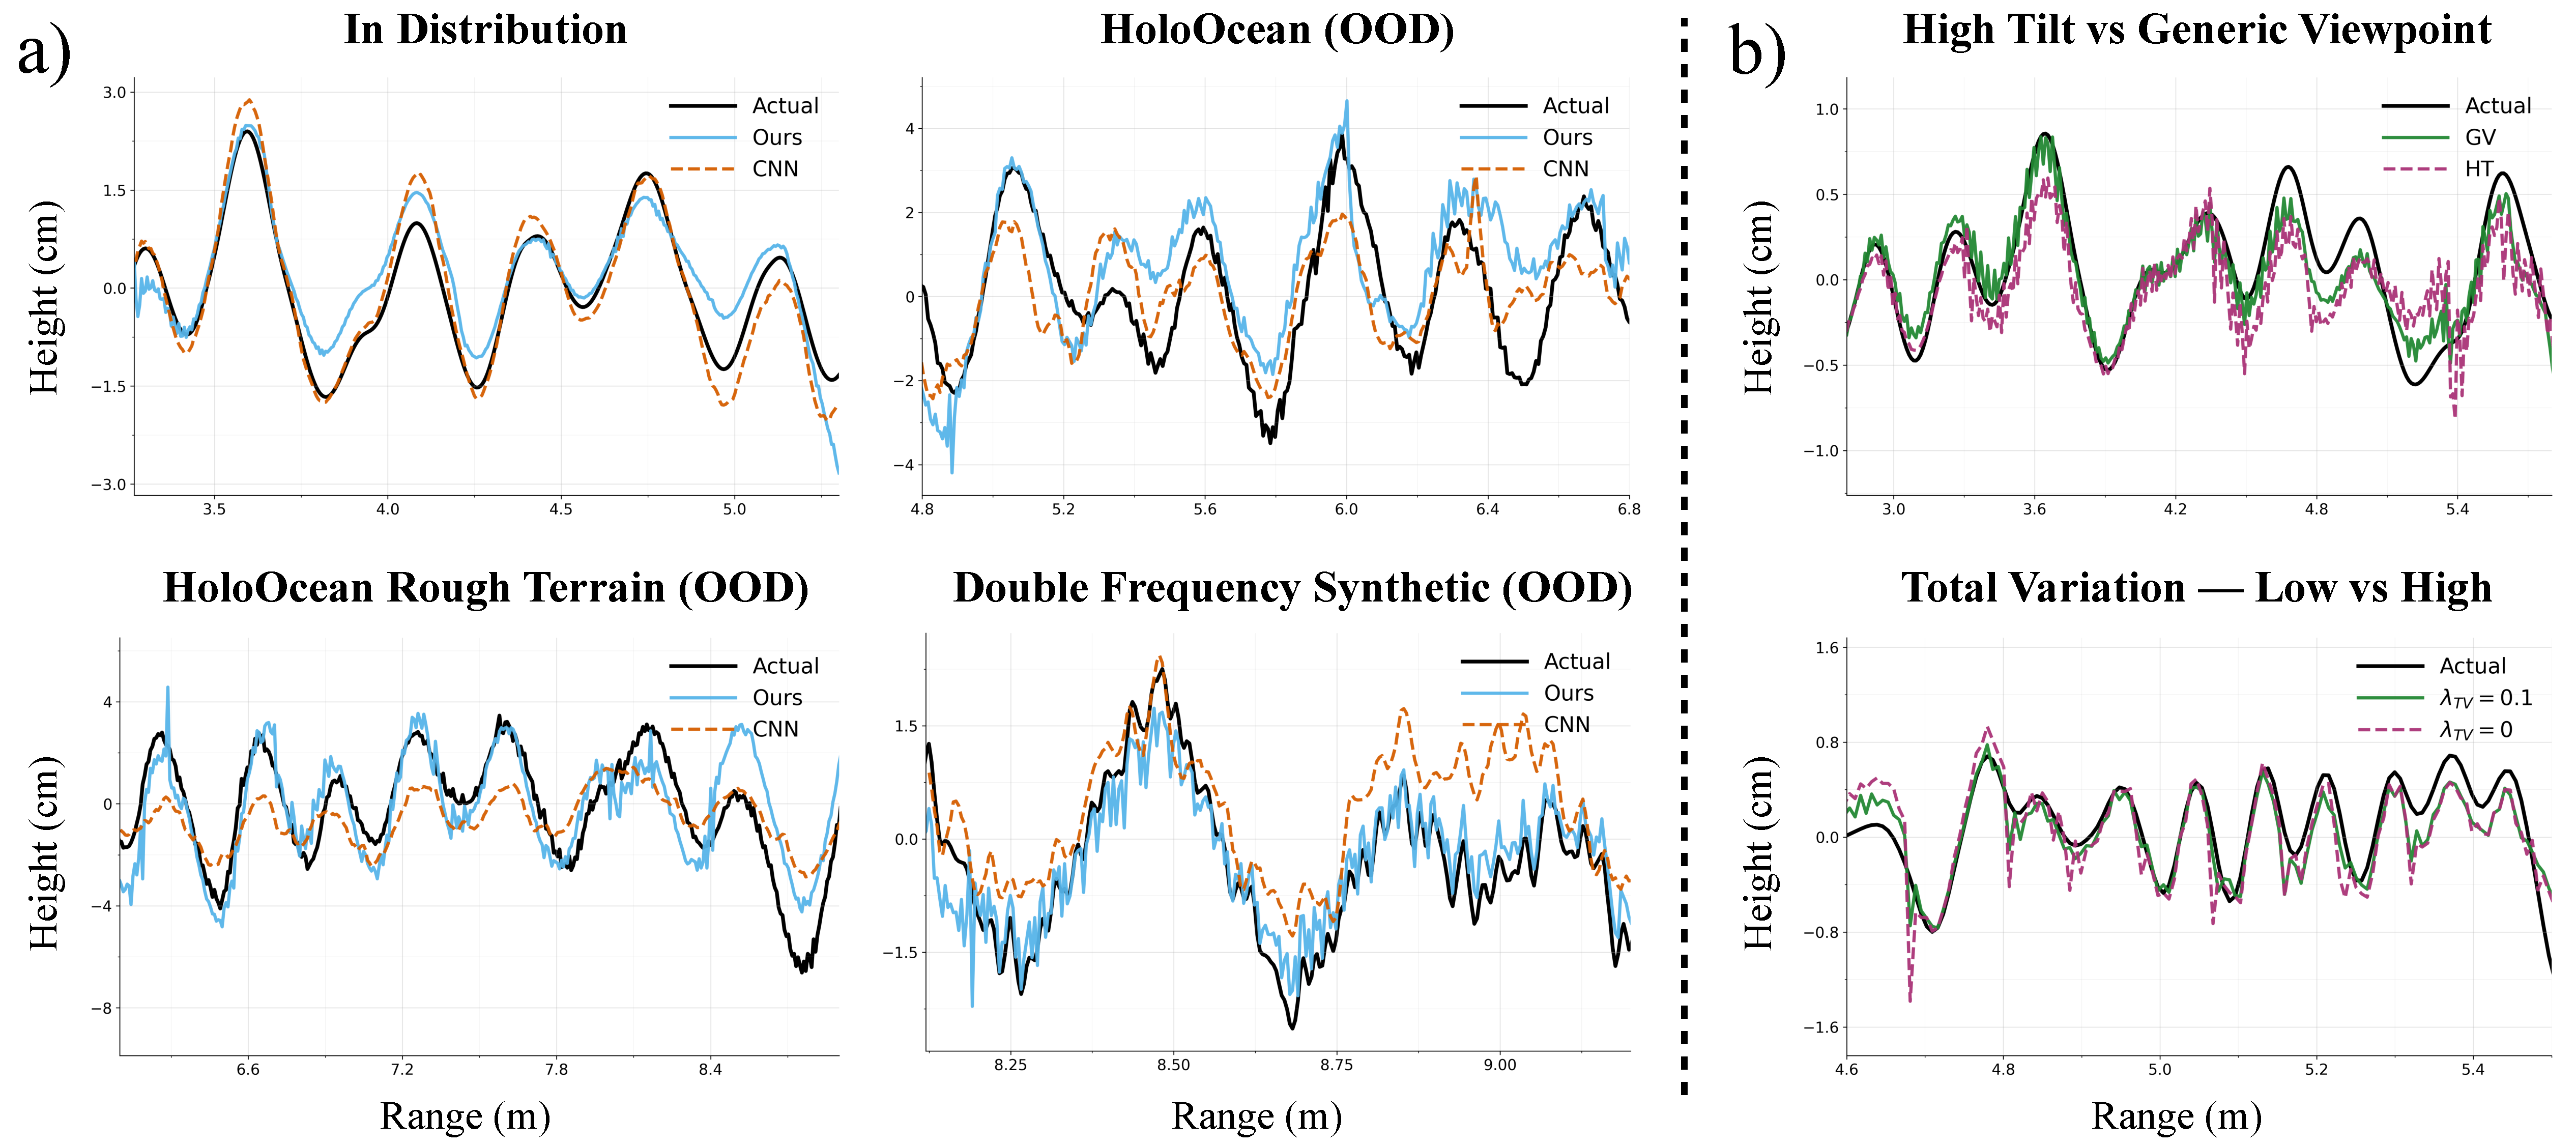
\includegraphics[width=1.0\linewidth]{figs/azimuth_preds.pdf}
\vspace{-0.2in}
   \caption{{\bf Heights predicted down a single azimuth beam as compared to the ground truth}. (a) Samples from each of our datasets, as well as a double-frequency case where we stack Perlin noise. (b) Comparisons between our generic viewpoint implementation and a fixed high-tilt plane, and low vs high TV regularization strengths. See Sec.~\ref{sec:qualitative} for details. \vspace{-4mm}}
   \label{fig:azimuth_preds}
\end{figure*}

\section{Experiments}
\label{sec:experiments}

We evaluate performance on synthetic datasets with known ground-truth elevations and compare against a supervised CNN baseline. {All methods are evaluated in a common 3D reference frame by converting predicted height deviations into point clouds defined on the ground-truth sonar sampling grid. We then report mean Chamfer distance (MCD) and 3D RMSE/MAE/MSE between point sets (\cref{sec:model_eval}).} Synthetic datasets are generated using a combination of our simulator and the HoloOcean sonar simulator built in Unreal Engine~\cite{2022PotokarHoloOcean,Romrell2025HoloOcean2}. We additionally test qualitative fits on real river imagery without ground-truth elevations.
 
\subsection{Synthetic In-Distribution Dataset}
\label{sec:in_dist_exp}
Using our simulator, we generated 10,000 training samples and 200 validation samples for training the CNN, and 200 testing samples to evaluate all methods. The training set was not used for our approach since we fit geometry on individual frames without pretraining. Seafloors were generated using Perlin noise with randomized frequency and centimeter-scale amplitudes added to a base-plane at randomized tilts. Each plane was chosen to ensure returns along the full sonar range. Each sample also had a randomized sonar configuration, including range, binning, azimuth coverage, and elevation angles. Ranges in consideration were \(<\)10m, and elevation coverage was chosen in the range of \(10-30^{\circ}\). Full dataset parameters are listed in the supplemental materials. Each validation sample input is comprised of the sensor reading and sonar configuration metadata. The target is a height-deviation map defined on the sample's sonar range–azimuth grid in the coordinate frame of the sample's base plane (\ie, conditioned on the known base-plane tilt).

\subsection{HoloOcean Datasets}
To evaluate out-of-distribution performance, we generated two additional test datasets using HoloOcean, each with samples in the same input-output format as in Sec.~\ref{sec:in_dist_exp}. In the first dataset we use a similar randomized Perlin noise and sonar configuration sampling scheme as the in-distribution data. We also generated a ``rough terrain'' dataset with increased amplitudes and range coverage, making the task more challenging. 

\subsection{Real River Fits}
Targets from real riverbeds were acquired using ARIS and Didson sonar cameras, with samples produced by averaging the frames over a clip to reduce noise and transitory objects. The corresponding configuration files were parsed to initialize our model with the proper beam directions, samples per beam, and range parameters. No processing is done to the raw target frames other than rescaling. Images were collected from a set of rivers near the U.S. West Coast.

\subsection{CNN Baseline}
For the CNN baseline, we use a standard U-Net with four encoder and four decoder stages (3$\times$3 conv--BN--ReLU blocks), a 1/16-resolution bottleneck with 1024 channels, and bilinear upsampling with skip connections to predict a single-channel height-deviation map. The model is trained for 200 epochs on 10{,}000 samples using MSE loss.

\subsection{Model Evaluation}
\label{sec:model_eval}

We evaluate models from their predicted height-deviation map on the range--azimuth grid by converting predictions and ground truth into 3D point clouds in a common coordinate frame. For each bin, we compute its 3D location on the base plane using the known tilt and sensor geometry, then offset along the local radial direction in the sensor's range–azimuth plane (\ie, along the constant-range arc at that bin).

\subsection{Implementation Details}
We implement our simulator using PyTorch~\cite{Paszke2019Pytorch} for autodiff., and we fit our seafloor height field by optimizing Eq.~\ref{eq:main_loss} using AdamW~\cite{2019LoshchilovAdamW} for 150 steps using a learning rate of \(1e-4\). Azimuth scaling factors have a learning rate of \(0\) until \(n_{\text{warmup}}=30\) steps when we raise it to \(0.1\). We set \(\lambda_{\text{TV}}=0.1\) by default. On an RTX 5090 our model achieves ~12 iterations per second, generating an image in under \(100\)ms. Fully fitting a 3D height field takes \(5-15\)s for \(150\) optimization steps, depending on target size.

In all synthetic experiments, the base-plane tilt is treated as known at evaluation time, and the CNN is trained and evaluated under the same assumption. We report three variants of our inverse method that differ only in the {optimization-time} plane orientation: known-plane (KP) uses the known tilt, high-tilt (HT) fixes a steep tilt for all samples, and generic-view (GV) resamples a new tilt each optimization step to encourage robust geometry.